\documentclass[aspectratio=169,10pt]{beamer}

\usepackage[utf8]{inputenc}
\usepackage[T1]{fontenc}
\usepackage[spanish,es-nodecimaldot,es-tabla]{babel}
\usepackage{csquotes}
\usepackage[sfdefault]{FiraSans}
\usepackage{inconsolata}
\usepackage{graphicx}
\usepackage{booktabs}
\usepackage{tabularx}
\usepackage{array}
\usepackage{colortbl}
\usepackage{xcolor}
\usepackage{tikz}
\usetikzlibrary{babel}
\usepackage[most]{tcolorbox}
\usepackage[backend=biber,style=ieee]{biblatex}
\addbibresource{referencias.bib}

\renewcommand*{\mkbibacro}[1]{#1}

% =====================================================================
% PALETA MODERNA (Midnight + Cobalt + Amber + Cool Slate)
% =====================================================================
\definecolor{NavyDark}{HTML}{0B1120}
\definecolor{NavySoft}{HTML}{1E293B}
\definecolor{BlueAccent}{HTML}{2563EB}
\definecolor{AmberAccent}{HTML}{D97706}
\definecolor{CardBg}{HTML}{F8FAFC}
\definecolor{CardBorder}{HTML}{CBD5E1}
\definecolor{SlateText}{HTML}{475569}
\definecolor{RowAlt}{HTML}{F1F5F9}

\usetheme{default}
\usecolortheme{default}
\setbeamertemplate{navigation symbols}{}
\setbeamertemplate{itemize item}{\textcolor{BlueAccent}{\small$\blacktriangleright$}}
\setbeamertemplate{frametitle continuation}{}

\setbeamercolor{normal text}{fg=NavyDark,bg=white}
\setbeamercolor{structure}{fg=BlueAccent}
\setbeamercolor{frametitle}{fg=NavyDark,bg=white}
\setbeamercolor{framesubtitle}{fg=SlateText}

\setbeamerfont{frametitle}{size=\Large,series=\bfseries}
\setbeamerfont{framesubtitle}{size=\footnotesize,series=\mdseries}

% Encabezado moderno con línea de acento degradada (azul -> gris)
\makeatletter
\setbeamertemplate{frametitle}{
  \nointerlineskip
  \begin{beamercolorbox}[wd=\paperwidth,ht=1.28cm,dp=0.20cm,leftskip=0.75cm,rightskip=0.75cm]{frametitle}
    \vspace{0.15cm}
    {\usebeamerfont{frametitle}\insertframetitle}\par
    \ifx\insertframesubtitle\@empty\else
      \vspace{0.05cm}
      {\usebeamerfont{framesubtitle}\insertframesubtitle}\par
    \fi
  \end{beamercolorbox}
  \nointerlineskip
  \hbox{\color{BlueAccent}\rule{2.8cm}{2pt}\color{CardBorder}\rule{\dimexpr\paperwidth-2.8cm\relax}{0.6pt}}
  \vspace{-0.15cm}
}
\makeatother

% Pie de página minimalista con píldora numerada
\setbeamertemplate{footline}{
  \leavevmode%
  \hbox{\color{CardBorder}\rule{\paperwidth}{0.5pt}}%
  \vspace{2pt}
  \hbox{%
    \begin{beamercolorbox}[wd=.78\paperwidth,ht=2.4ex,dp=1.2ex,leftskip=0.75cm]{author in head/foot}%
      \textcolor{SlateText}{\scriptsize Equipo EJPZ \;\textbullet\; Aplicaciones Distribuidas (Paralelo A) \;\textbullet\; UTEQ}
    \end{beamercolorbox}%
    \begin{beamercolorbox}[wd=.22\paperwidth,ht=2.4ex,dp=1.2ex,rightskip=0.75cm]{date in head/foot}%
      \hfill\textcolor{BlueAccent}{\scriptsize\bfseries \insertframenumber}\textcolor{SlateText}{\scriptsize\ / \inserttotalframenumber}
    \end{beamercolorbox}%
  }%
  \vskip2pt%
}

% =====================================================================
% TARJETAS MODERNAS (tcolorbox)
% =====================================================================
\newtcolorbox{bluecard}[1]{
  enhanced,
  colback=CardBg,
  colframe=CardBorder,
  boxrule=0.6pt,
  arc=4pt,
  borderline north={2.8pt}{0pt}{BlueAccent},
  title={#1},
  coltitle=BlueAccent,
  colbacktitle=CardBg,
  fonttitle=\bfseries\normalsize,
  halign title=flush left,
  halign=flush left,
  titlerule=0.4pt,
  titlerule style={CardBorder},
  toptitle=4pt, bottomtitle=4pt,
  left=8pt, right=8pt, top=6pt, bottom=6pt
}

\newtcolorbox{ambercard}[1]{
  enhanced,
  colback=CardBg,
  colframe=CardBorder,
  boxrule=0.6pt,
  arc=4pt,
  borderline north={2.8pt}{0pt}{AmberAccent},
  title={#1},
  coltitle=AmberAccent,
  colbacktitle=CardBg,
  fonttitle=\bfseries\normalsize,
  halign title=flush left,
  halign=flush left,
  titlerule=0.4pt,
  titlerule style={CardBorder},
  toptitle=4pt, bottomtitle=4pt,
  left=8pt, right=8pt, top=6pt, bottom=6pt
}

\newtcolorbox{demobar}{
  enhanced,
  colback=NavyDark,
  colframe=NavyDark,
  coltext=white,
  arc=4pt,
  borderline west={3.5pt}{0pt}{AmberAccent},
  halign=flush left,
  left=10pt, right=10pt, top=5pt, bottom=5pt,
  fontupper=\footnotesize
}

\title{WebSockets, TCP y UDP en JobFinder}
\subtitle{Comunicación en tiempo real aplicada a la Bolsa de Empleos para Graduados}
\author{Kenny España \and Luis Jaramillo \and Luis Paca \and Heiner Zambrano}
\institute{Equipo EJPZ --- Facultad de Ciencias de la Computación, UTEQ}
\date{Noviembre 2026}

\begin{document}

% =====================================================================
% DIAPOSITIVA 1: PORTADA KEYNOTE FULL-BLEED
% =====================================================================
\begin{frame}[plain]
  \begin{tikzpicture}[remember picture,overlay]
    \fill[NavyDark] (current page.south west) rectangle (current page.north east);
    \fill[BlueAccent] (current page.south west) rectangle ([xshift=0.35cm]current page.north west);
    \fill[AmberAccent] ([xshift=0.35cm,yshift=-0.12cm]current page.north west) rectangle ([xshift=4.2cm]current page.north west);
    \fill[NavySoft,opacity=0.45] ([xshift=-3.6cm]current page.north east) -- (current page.north east) -- (current page.south east) -- ([xshift=-1.4cm]current page.south east) -- cycle;
  \end{tikzpicture}
  \vspace{1.2cm}
  \hspace{0.5cm}\begin{minipage}{0.86\textwidth}
    {\footnotesize\bfseries\textcolor{AmberAccent}{APLICACIONES DISTRIBUIDAS \;\textbullet\; PARALELO A \;\textbullet\; UTEQ}}\par
    \vspace{0.45cm}
    {\Huge\bfseries\textcolor{white}{WebSockets, TCP y UDP\\en JobFinder}}\par
    \vspace{0.35cm}
    {\large\textcolor{CardBorder}{Comunicación en tiempo real aplicada a la Bolsa de Empleos para Graduados}}\par
    \vspace{1.15cm}
    {\color{BlueAccent}\rule{2.2cm}{1.5pt}}\par
    \vspace{0.35cm}
    {\footnotesize\textcolor{white}{\textbf{Equipo EJPZ:} Kenny España \;\textbullet\; Luis Jeremy Jaramillo \;\textbullet\; Heiner Zambrano \;\textbullet\; Luis Alberto Paca}}\par
    \vspace{0.12cm}
    {\scriptsize\textcolor{CardBorder}{Facultad de Ciencias de la Computación --- Universidad Técnica Estatal de Quevedo}}
  \end{minipage}
\end{frame}

% =====================================================================
% DIAPOSITIVA 2: 1. PRESENTACIÓN DEL SISTEMA (KENNY ESPAÑA)
% =====================================================================
\begin{frame}{1. Presentación del Sistema (Kenny España)}
  \framesubtitle{Inserción laboral en la UTEQ y alcance de JobFinder \cite{uteq2022seguimiento}}
  \vspace{0.15cm}
  \begin{columns}[T,totalwidth=\textwidth]
    \begin{column}{0.315\textwidth}
      \begin{bluecard}{Empleabilidad Actual}
        \centering
        \vspace{0.15cm}
        {\Huge\bfseries\textcolor{BlueAccent}{51,50\,\%}}\par
        \vspace{0.2cm}
        \footnotesize Graduados con empleo activo según informe UTEQ \cite{uteq2022seguimiento}.
      \end{bluecard}
    \end{column}
    \begin{column}{0.315\textwidth}
      \begin{ambercard}{Canal Institucional}
        \centering
        \vspace{0.15cm}
        {\Huge\bfseries\textcolor{AmberAccent}{8,41\,\%}}\par
        \vspace{0.2cm}
        \footnotesize Contratados mediante bolsas de empleo universitarias \cite{uteq2022seguimiento}.
      \end{ambercard}
    \end{column}
    \begin{column}{0.315\textwidth}
      \begin{bluecard}{Actores del Sistema}
        \centering
        \vspace{0.15cm}
        {\Huge\bfseries\textcolor{NavyDark}{3 Roles}}\par
        \vspace{0.2cm}
        \footnotesize Graduado, Empresa Colaboradora y Administrador UTEQ.
      \end{bluecard}
    \end{column}
  \end{columns}
  \vspace{0.45cm}
  \begin{demobar}
    \textcolor{AmberAccent}{\textbf{Propósito:}} Centralizar vacantes validadas por administradores y ofertas externas sincronizadas para los graduados de la UTEQ \cite{ref1}.
  \end{demobar}
\end{frame}

% =====================================================================
% DIAPOSITIVA 3: TCP VS UDP (KENNY ESPAÑA)
% =====================================================================
\begin{frame}{Protocolos TCP frente a UDP (Kenny España)}
  \framesubtitle{Fundamento de la capa de transporte \cite{ref2,guo2025tcpudp}}
  \vspace{0.2cm}
  \begin{columns}[T,totalwidth=\textwidth]
    \begin{column}{0.485\textwidth}
      \begin{bluecard}{TCP --- Adoptado en JobFinder}
        \begin{itemize}\setlength{\itemsep}{6pt}
          \item \textbf{Conexión:} saludo de tres vías (\textit{three-way handshake}).
          \item \textbf{Fiabilidad:} entrega ordenada y acuses \texttt{ACK}.
          \item \textbf{Uso:} postulaciones y alertas críticas.
        \end{itemize}
      \end{bluecard}
    \end{column}
    \begin{column}{0.485\textwidth}
      \begin{ambercard}{UDP --- Descartado}
        \begin{itemize}\setlength{\itemsep}{6pt}
          \item \textbf{Conexión:} datagramas sin sesión previa.
          \item \textbf{Fiabilidad:} sin retransmisión ante pérdidas.
          \item \textbf{Uso:} multimedia o telemetría tolerante a fallos.
        \end{itemize}
      \end{ambercard}
    \end{column}
  \end{columns}
\end{frame}

% =====================================================================
% DIAPOSITIVA 4: CICLO WEBSOCKET + PRÁCTICA 1 (KENNY ESPAÑA)
% =====================================================================
\begin{frame}{Ciclo WebSocket (RFC 6455) y Práctica 1 (Kenny España)}
  \framesubtitle{Establecimiento del canal Full-Duplex sobre TCP \cite{ref3,mitrovic2023websocket}}
  \vspace{0.2cm}
  \begin{columns}[T,totalwidth=\textwidth]
    \begin{column}{0.235\textwidth}
      \begin{bluecard}{01. Petición}
        \footnotesize Cliente envía \texttt{Upgrade: websocket} sobre HTTP.
      \end{bluecard}
    \end{column}
    \begin{column}{0.235\textwidth}
      \begin{bluecard}{02. HTTP 101}
        \footnotesize Servidor acepta con \texttt{101 Switching Protocols}.
      \end{bluecard}
    \end{column}
    \begin{column}{0.235\textwidth}
      \begin{bluecard}{03. Full-Duplex}
        \footnotesize Tramas ligeras bidireccionales sobre TCP.
      \end{bluecard}
    \end{column}
    \begin{column}{0.235\textwidth}
      \begin{ambercard}{04. Práctica 1}
        \footnotesize Envío UDP vs. sesión WS en DevTools.
      \end{ambercard}
    \end{column}
  \end{columns}
  \vspace{0.5cm}
  \begin{demobar}
    \textcolor{AmberAccent}{\textbf{Demostración en vivo:}} Ejecución de \texttt{demo\_udp.js} en terminal y verificación de \texttt{HTTP 101} en Chrome DevTools.
  \end{demobar}
\end{frame}

% =====================================================================
% DIAPOSITIVA 5: 2. ARQUITECTURA REAL (LUIS JEREMY JARAMILLO)
% =====================================================================
\begin{frame}{2. Arquitectura del Sistema JobFinder (Luis Jeremy Jaramillo)}
  \framesubtitle{Angular (:4200) \;\textbullet\; Spring Boot (:8080) \;\textbullet\; PostgreSQL (:5432) + Full-Duplex}
  \centering
  \vspace{0.08cm}
  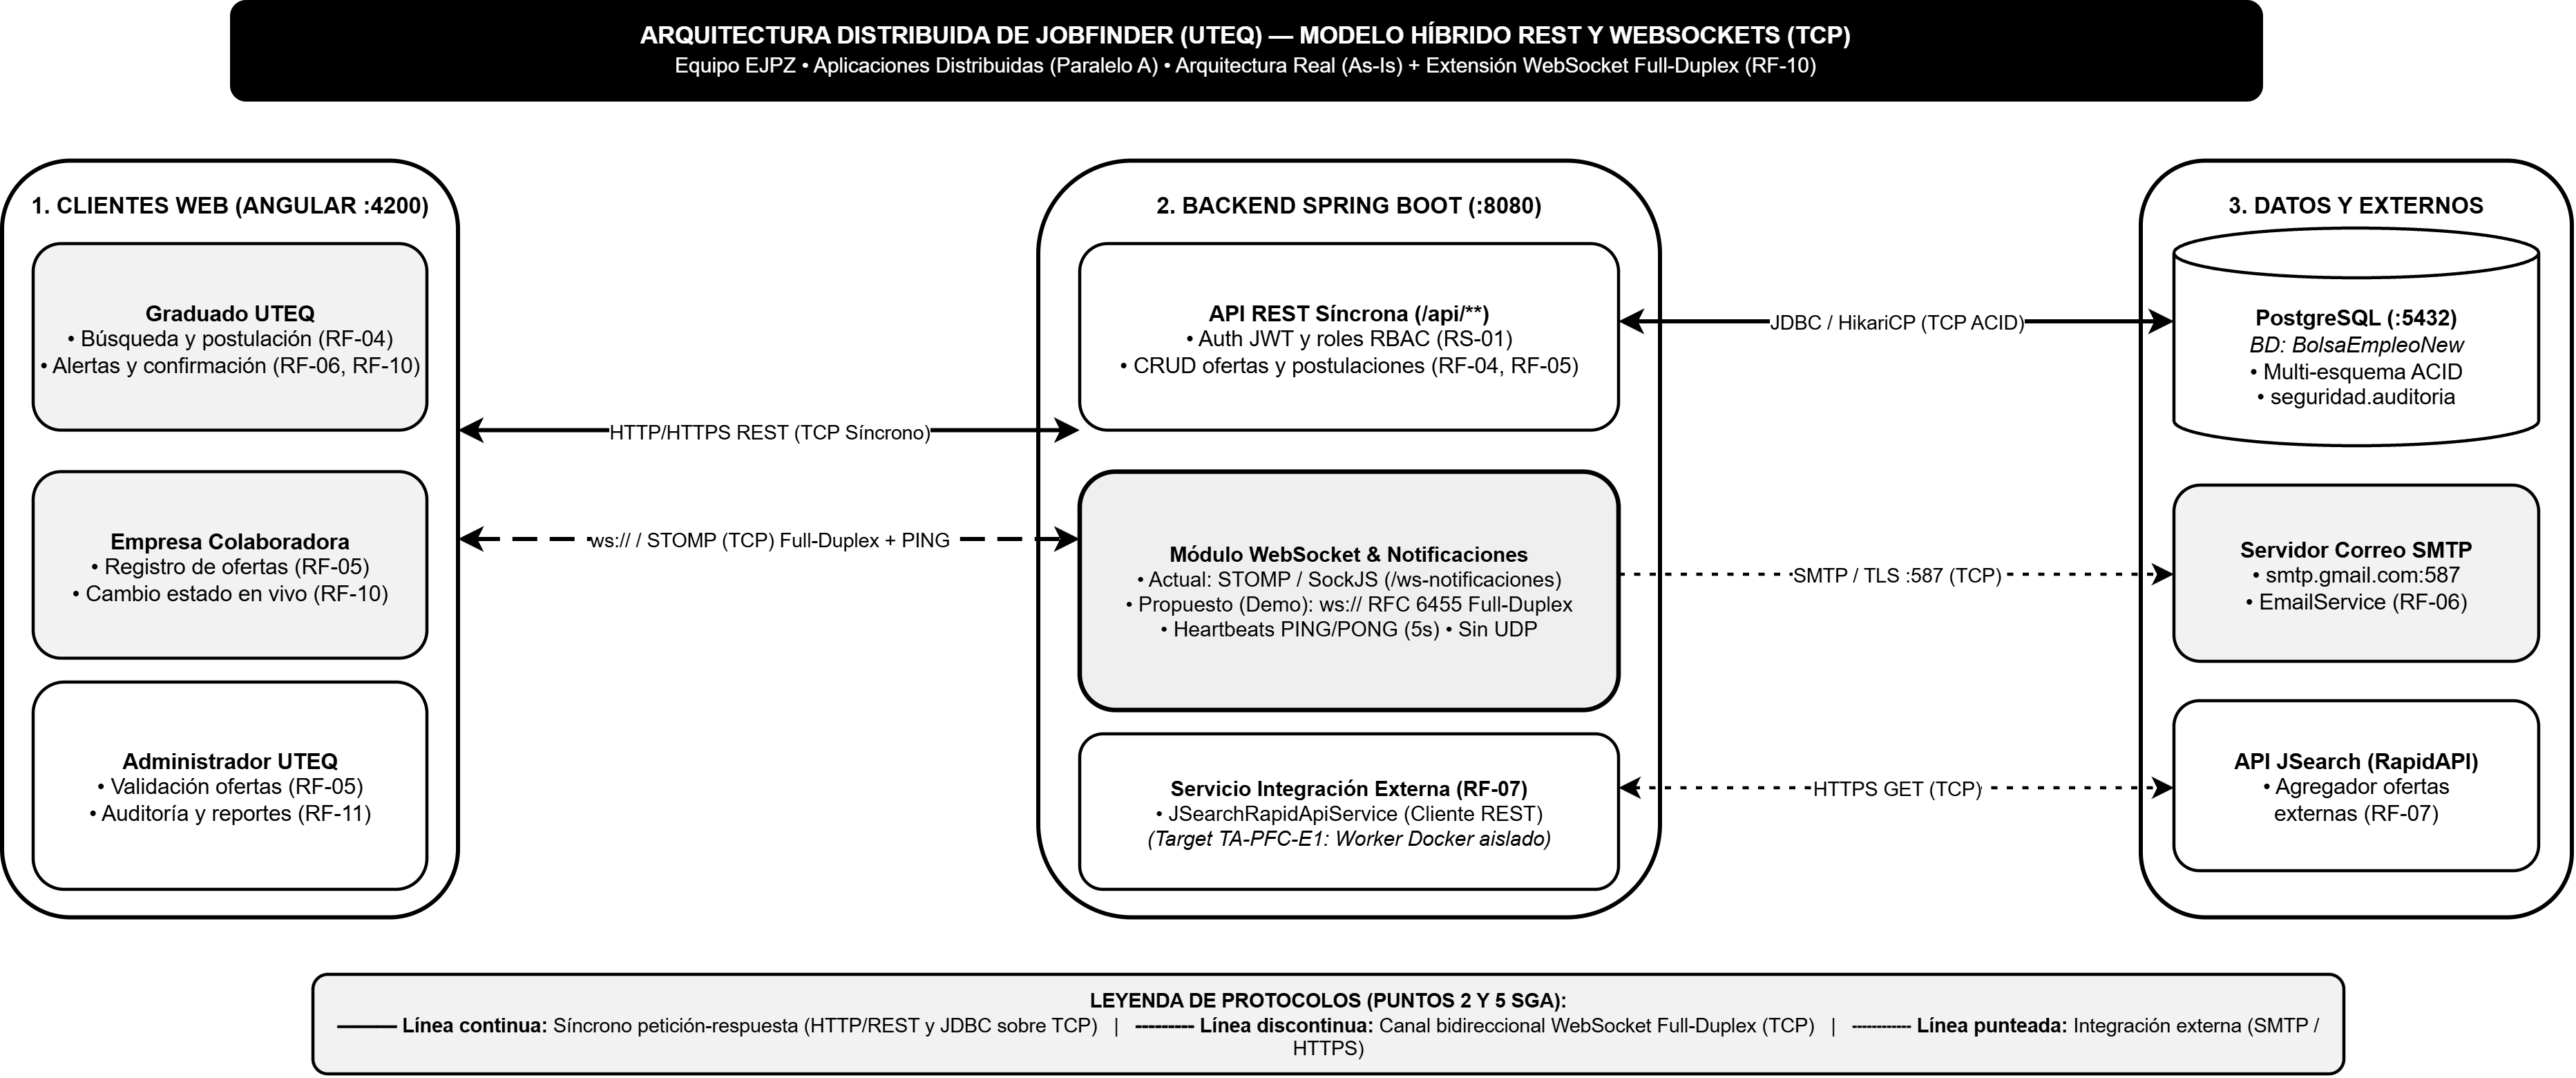
\includegraphics[width=0.90\textwidth,height=0.55\textheight,keepaspectratio]{arquitectura_jobfinder.png}\par
  \vspace{0.18cm}
  \begin{demobar}
    \textcolor{AmberAccent}{\textbf{Deuda técnica (Arquitectura):}} \texttt{JSearchRapidApiService} corre síncrono dentro de \texttt{:8080}; en el PFC (\texttt{TA-PFC-E1}) se aísla en un \textit{worker} Docker con contratos retrocompatibles \cite{ref4}.
  \end{demobar}
\end{frame}

% =====================================================================
% DIAPOSITIVA 6: 5. MODELOS DE COMUNICACIÓN + PRÁCTICA 2 (JEREMY — LIMPIA)
% =====================================================================
\begin{frame}{5. Modelos de Comunicación y Práctica 2 (Luis Jeremy Jaramillo)}
  \framesubtitle{Cliente--servidor híbrido sobre TCP: puntos clave en Spring Boot \cite{ref3,ref4,petrescu2025iotprotocols}}
  \vspace{0.10cm}
  \begin{columns}[T,totalwidth=\textwidth]
    \begin{column}{0.485\textwidth}
      \begin{bluecard}{REST Síncrono (\texttt{/api/**})}
        \footnotesize
        \begin{itemize}\setlength{\itemsep}{5pt}
          \item \textbf{Núcleo HTTP/TCP:} JWT/RBAC (\texttt{RS-01}), validación (\texttt{RF-05}) y postulación (\texttt{RF-04}).
          \item \textbf{Evaluación:} \texttt{@PostMapping} síncrono y auditable.
          \item \textbf{Externo (\texttt{RF-07}):} \texttt{HttpClient} a RapidAPI (futuro desacoplo AMQP \cite{petrescu2025iotprotocols}).
        \end{itemize}
      \end{bluecard}
    \end{column}
    \begin{column}{0.485\textwidth}
      \begin{ambercard}{WebSocket (\texttt{/ws-notificaciones})}
        \footnotesize
        \begin{itemize}\setlength{\itemsep}{5pt}
          \item \textbf{Bróker STOMP:} \texttt{/app}, \texttt{/topic}, \texttt{/queue} y respaldo \texttt{withSockJS()}.
          \item \textbf{Full-Duplex (\texttt{RF-10}):} \texttt{@MessageMapping} + \texttt{@Transactional} (\texttt{Entrevista OK}) \cite{mitrovic2023websocket}.
          \item \textbf{Por qué WS:} supera a \textit{polling} HTTP y a SSE (solo unidireccional).
        \end{itemize}
      \end{ambercard}
    \end{column}
  \end{columns}
  \vspace{0.25cm}
  \begin{demobar}
    \textcolor{AmberAccent}{\textbf{Práctica 2 en vivo:}} Recorrido de código real (4 clases Spring Boot) $\rightarrow$ flujo \texttt{RF-10} inspeccionando tramas bidireccionales en DevTools (\texttt{Network} $\rightarrow$ \texttt{WS} $\rightarrow$ \texttt{Messages}).
  \end{demobar}
\end{frame}

% =====================================================================
% DIAPOSITIVA 7: 3. TRANSPARENCIAS DE DISTRIBUCIÓN (HEINER ZAMBRANO)
% =====================================================================
\begin{frame}{3. Transparencias de Distribución (Heiner Zambrano)}
  \framesubtitle{Propiedades garantizadas y limitaciones en JobFinder}
  \vspace{0.12cm}
  \begin{columns}[T,totalwidth=\textwidth]
    \begin{column}{0.485\textwidth}
      \begin{bluecard}{Acceso Unificado (SÍ)}
        \footnotesize Rutas \texttt{/api/**} y \texttt{/ws-notificaciones} abstraen protocolos internos.
      \end{bluecard}
      \vspace{0.25cm}
      \begin{bluecard}{Concurrencia Activa (SÍ)}
        \footnotesize Múltiples sesiones WebSocket en paralelo + ACID en PostgreSQL.
      \end{bluecard}
    \end{column}
    \begin{column}{0.485\textwidth}
      \begin{bluecard}{Ubicación Oculta (SÍ)}
        \footnotesize Puertos internos (\texttt{:5432}, \texttt{:8080}, \texttt{:587}) invisibles al cliente.
      \end{bluecard}
      \vspace{0.25cm}
      \begin{ambercard}{Fallos Explícitos (NO)}
        \footnotesize Cortes abruptos en red móvil exigen reconexión visible del cliente.
      \end{ambercard}
    \end{column}
  \end{columns}
\end{frame}

% =====================================================================
% DIAPOSITIVA 8: 4. CAP Y PACELC + PRÁCTICA 3 (HEINER ZAMBRANO)
% =====================================================================
\begin{frame}{4. Teoremas CAP y PACELC (Heiner Zambrano)}
  \framesubtitle{Compromiso entre consistencia, disponibilidad y latencia \cite{ref5}}
  \vspace{0.15cm}
  \begin{columns}[T,totalwidth=\textwidth]
    \begin{column}{0.485\textwidth}
      \begin{bluecard}{CP --- Con Partición de Red (P)}
        \textbf{Prioridad: Consistencia (C)}\par
        \vspace{0.15cm}
        \footnotesize Ante pérdida de enlace con \texttt{BolsaEmpleoNew}, se bloquean escrituras de postulación para evitar duplicados o vacantes sin validar.
      \end{bluecard}
    \end{column}
    \begin{column}{0.485\textwidth}
      \begin{ambercard}{EL / EC --- Operación Normal (E)}
        \textbf{Prioridad: Latencia (L) y Consistencia (C)}\par
        \vspace{0.15cm}
        \footnotesize Sin particiones, prioriza baja latencia en alertas WebSocket (\textbf{PA/EL}) e integridad ACID multi-esquema en PostgreSQL (\textbf{PC/EC}).
      \end{ambercard}
    \end{column}
  \end{columns}
  \vspace{0.4cm}
  \begin{demobar}
    \textcolor{AmberAccent}{\textbf{Práctica 3 en vivo:}} Partición hacia PostgreSQL (\texttt{:5432}) bloqueando escrituras (\texttt{BLOQUEO CAP}) mientras lectura en caché responde en $< 5$\,ms.
  \end{demobar}
\end{frame}

% =====================================================================
% DIAPOSITIVA 9: 6. TOLERANCIA A FALLOS + PRÁCTICA 4 (LUIS ALBERTO PACA)
% =====================================================================
\begin{frame}{6. Tolerancia a Fallos y Práctica 4 (Luis Alberto Paca)}
  \framesubtitle{Detección activa, aislamiento y recuperación escalonada \cite{mitrovic2023websocket,ref4}}
  \vspace{0.15cm}
  \begin{columns}[T,totalwidth=\textwidth]
    \begin{column}{0.315\textwidth}
      \begin{bluecard}{Heartbeats PING/PONG}
        \footnotesize Sondeo TCP activo cada 5\,s para detectar y liberar sockets inactivos.
      \end{bluecard}
    \end{column}
    \begin{column}{0.315\textwidth}
      \begin{bluecard}{Aislamiento FORM-AC-01}
        \footnotesize Desacoplar la consulta externa (\texttt{RF-07}) evita bloqueos en cascada del servidor.
      \end{bluecard}
    \end{column}
    \begin{column}{0.315\textwidth}
      \begin{ambercard}{Backoff Exponencial}
        \footnotesize Reintentos escalonados en 1\,s, 2\,s, 4\,s y 8\,s tras una caída del backend.
      \end{ambercard}
    \end{column}
  \end{columns}
  \vspace{0.45cm}
  \begin{demobar}
    \textcolor{AmberAccent}{\textbf{Práctica 4 en vivo:}} Detención forzada del servidor WebSocket (\texttt{Ctrl+C}) y reconexión automática escalonada al reiniciar.
  \end{demobar}
\end{frame}

% =====================================================================
% DIAPOSITIVA 10: 7. COMPARACIÓN Y POSTURA CRÍTICA (LUIS ALBERTO PACA)
% =====================================================================
\begin{frame}{7. Comparación y Postura Crítica (Luis Alberto Paca)}
  \framesubtitle{JobFinder frente a portales laborales comerciales \cite{linkedinFeedInfra,linkedin2025northguard,ref1}}
  \vspace{0.15cm}
  \begin{tcolorbox}[enhanced,colback=white,colframe=CardBorder,boxrule=0.6pt,arc=4pt,left=4pt,right=4pt,top=4pt,bottom=4pt]
    \small
    \renewcommand{\arraystretch}{1.35}
    \begin{tabularx}{\linewidth}{@{}>{\bfseries\color{NavyDark}\raggedright\arraybackslash}p{3.4cm}>{\raggedright\arraybackslash}X>{\raggedright\arraybackslash}X@{}}
      \rowcolor{NavyDark}
      \textcolor{white}{Criterio Técnico} & \textcolor{white}{\textbf{JobFinder UTEQ}} & \textcolor{white}{\textbf{LinkedIn / CompuTrabajo}} \\
      Validación de ofertas & Control administrativo previo (\texttt{RF-05}) & Publicación abierta sin filtro institucional \\
      \rowcolor{RowAlt}
      Notificaciones & Push bidireccional vía WebSockets & Correo electrónico o consulta periódica \\
      Pertinencia curricular & Filtrado por carreras de la UTEQ & Ofertas genéricas masivas \\
      \rowcolor{RowAlt}
      Compromiso (\textit{Trade-off}) & Mayor RAM por sockets TCP abiertos & Menor memoria en APIs sin estado \\
    \end{tabularx}
  \end{tcolorbox}
\end{frame}

% =====================================================================
% DIAPOSITIVA 11: 8. LECCIONES PARA EL PFC (LUIS ALBERTO PACA)
% =====================================================================
\begin{frame}{8. Lecciones para el PFC y Conclusiones (Luis Alberto Paca)}
  \framesubtitle{Controles arquitectónicos para la entrega TA-PFC-E1 \cite{ref4,petrescu2025iotprotocols}}
  \vspace{0.15cm}
  \begin{columns}[T,totalwidth=\textwidth]
    \begin{column}{0.315\textwidth}
      \begin{bluecard}{Contenedores Aislados}
        \footnotesize Migrar la integración externa (\texttt{RF-07}) a un \textit{worker} Docker con colas AMQP.
      \end{bluecard}
    \end{column}
    \begin{column}{0.315\textwidth}
      \begin{bluecard}{Control de Sesiones}
        \footnotesize Configurar tramas \texttt{PING/PONG}, \textit{timeouts} y límites de tasa por socket TCP.
      \end{bluecard}
    \end{column}
    \begin{column}{0.315\textwidth}
      \begin{ambercard}{Auditoría Externa}
        \footnotesize Desacoplar registros de \texttt{seguridad.auditoria} y respaldos de la red pública.
      \end{ambercard}
    \end{column}
  \end{columns}
  \vspace{0.45cm}
  \begin{demobar}
    \textcolor{AmberAccent}{\textbf{Conclusión:}} WebSockets sobre TCP ofrece el equilibrio óptimo entre baja latencia y entrega ordenada para seguimiento laboral en tiempo real.
  \end{demobar}
\end{frame}

% =====================================================================
% DIAPOSITIVA 12: REFERENCIAS BIBLIOGRÁFICAS (IEEE)
% =====================================================================
\begin{frame}[allowframebreaks]{Referencias Bibliográficas (Formato IEEE)}
  \framesubtitle{Fuentes verificadas del estudio}
  \renewcommand*{\bibfont}{\scriptsize}
  \printbibliography[heading=none]
\end{frame}

% =====================================================================
% DIAPOSITIVA 13: CIERRE KEYNOTE FULL-BLEED
% =====================================================================
\begin{frame}[plain]
  \begin{tikzpicture}[remember picture,overlay]
    \fill[NavyDark] (current page.south west) rectangle (current page.north east);
    \fill[BlueAccent] (current page.south west) rectangle ([xshift=0.35cm]current page.north west);
    \fill[AmberAccent] ([xshift=-4.2cm,yshift=0.12cm]current page.south east) rectangle (current page.south east);
    \fill[NavySoft,opacity=0.45] ([xshift=-3.6cm]current page.north east) -- (current page.north east) -- (current page.south east) -- ([xshift=-1.4cm]current page.south east) -- cycle;
  \end{tikzpicture}
  \vspace{2.0cm}
  \centering
  {\footnotesize\bfseries\textcolor{AmberAccent}{9. DEFENSA TÉCNICA \;\textbullet\; EQUIPO EJPZ}}\par
  \vspace{0.4cm}
  {\Huge\bfseries\textcolor{white}{Preguntas y Discusión}}\par
  \vspace{0.55cm}
  {\color{BlueAccent}\rule{2.4cm}{1.5pt}}\par
  \vspace{0.55cm}
  {\normalsize\textcolor{white}{Kenny España \;\textbullet\; Luis Jeremy Jaramillo \;\textbullet\; Heiner Zambrano \;\textbullet\; Luis Alberto Paca}}\par
  \vspace{0.2cm}
  {\footnotesize\textcolor{CardBorder}{Aplicaciones Distribuidas (Paralelo A) \;\textbullet\; Facultad de Ciencias de la Computación --- UTEQ}}
\end{frame}

\end{document}